\documentclass[a4paper]{article}

%% Language and font encodings
\usepackage[english]{babel}
\usepackage[utf8x]{inputenc}

\usepackage[T1]{fontenc}
\usepackage{wrapfig, blindtext}

%% Sets page size and margins
\usepackage[a4paper,top=3cm,bottom=2cm,left=3cm,right=3cm,marginparwidth=1.75cm]{geometry}

%% Useful packages
\usepackage{amsmath}
\usepackage{graphicx}
\usepackage[colorinlistoftodos]{todonotes}
%Color a las referencias
\usepackage[colorlinks=true, allcolors=blue]{hyperref}
%Color a los textos

%Caratula
\begin{document}
\begin{titlepage}
\begin{center}
\vspace*{-0.4in}

{\fontsize{12}{30}\bf \selectfont UNIVERSIDAD NACIONAL DE INGENIERIA\\}

{\fontsize{12}{40}\bf \selectfont FACULTAD DE CIENCIAS\\}
\vspace*{0.15in} CIENCIAS DE LA COMPUTACI\'ON\\
\vspace*{0.2in}


\begin{center}

\includegraphics[width=5.5cm,height=6.5cm]{UNI.png}
\end{center}
\vspace*{0.2in}

\begin{large}
	{\bf PROYECTO DE BIOLOGIA COMPUTACIONAL\\}
	\vspace*{0.3in}
\end{large}

\begin{large}
{\bf T\'itulo del Trabajo\\}
\vspace*{0.2in}
\end{large}

\begin{Large}
\color{blue}
\textbf{Creación de un sistema de ayuda para el analisis de información Genética de Especies endémicas de las regiones del Perú\\}
\color{black}
\end{Large}
\vspace*{0.2in}

\begin{large}
{\bf Autores} 
\vspace*{0.1in}
\\L\'azaro Camasca, Edson Nicks\\
Leon Rios, Marco Naro
\end{large}
\vspace*{0.4in}


\begin{large}
{\bf Profesor} 
\vspace*{0.1in}
\\Nuñez Iturri, Ciro Javier
\end{large}

\end{center}
\begin{center}
\begin{large}
\vspace*{1.0in}
Lima - Peru\\
{\bf (2019)}
\end{large}
\end{center}
\end{titlepage}

\pagebreak
\tableofcontents
\pagebreak

\section{Objetivos}

\subsection{Objetivos Generales}
\begin{itemize}
\item  Creación de una aplicación gráfico con una base de datos para el análisis de información genética.
\end{itemize}

\subsection{Objetivos Específicos}

\begin{itemize}
\item Recolectar información genética de especies endémicas.
\item Desarrollar la aplicación para el análisis de secuencias,.
\item Desarrollar algoritmos para obtener árboles filogenéticos 
\item Evaluar el árbol filogenético
\end{itemize}

\section{Resumen Ejecutivo}

Se pretender crear una aplicación y una base de datos con la información genética de las especies endémicas del Perú, el software procesara las secuencias, creará el árbol filogenético, mostrará los resultados y analizará las relaciones evolutivas de las especies escogidas.

\section{Descripción del Proyecto}

El proyecto sera implementado netamente en el lenguaje Python
Las librerías utilizadas serán:
\begin{itemize}
\item BioPython para el procesamiento de secuencias
\item Flask para el entorno gráfico.
\end{itemize}
Dentro de la GUI, se pobre escoger Especies para el análisis posterior.\\
Los datos recolectados serán reales de la base de datos de NCBI.\\
Se implementara algoritmos para el alineamiento de Genes homólogos.\\
Se implementara algoritmos para el alineamiento de Proteínas.\\
Se implementara la algoritmos para la Generación de Arboles Filogenéticos de acuerdo a un modelo.\\

\noindent Para el desarrollo del proyecto se seguirá la siguiente metodología:

\subsection{Determinar las especies y el material a utilizar}
Se escogió las siguientes especies:
\begin{itemize}
    \item Tremarctos ornatus
    \item Panthera onca
    \item Vicugna vicugna
    \item Aulacorhynchus huallagae
    \item Leopardus jacobita
    \item Inia geoffrensis
    \item Spheniscus humboldti
    \item Vultur gryphus
    \item Lama glama
    \item Cavia porcellus
    \item Platalea ajaja
\end{itemize}

Estas especies se escogieron por ser especies endémicas del Perú, especias en peligro de extinción en el Perú y especies representativas del Perú. Además, se tuvo en cuenta la disponibilidad de material genético puesto que muchas de las especies endémicas poseen una base de datos genética incompleta y algunas no se encuentran codificadas en absoluto.

La proteína a analizarse sera el NADH deshidrogenasa, también conocido como Complejo I, subunidad 2 debido a que se encuentra presente en todas las especias y está codificado. 
La proteína escogida cumple una importante función en la respiración bacteriana y mitocondrial. Por ende, es posible encontrarla en diversas especies y no es extraño que se haya codificado.
Una importante observación es que no todas las especies se encuentran codificadas en la base de datos de NCBI, faltando genes importantes.
\subsection{Elegir los marcadores moleculares}
\subsection{Realizar el lineamiento múltiple de genes homólogos}
\subsection{Elegir un modelo evolutivo}
Entre los modelos tenemos:

\begin{itemize}
\item Modelo Jukes-Cantor: asimiento que los nucleótidos son substituidos con igual probabilidad
\item Modelo Kimura: realista ya que considera las diferentes tasas de mutación
\end{itemize}
\subsection{Aplicar un método para la construcción del árbol filogenético}	
Entre los métodos tenemos 
\begin{itemize}
	\item Basados en distancia
	\item Basados en secuencia
	\item Basados en agrupamiento
	\item Basados en optimalidad
	\item Basados en caracteres
\end{itemize}

\subsection{Verificar la fiabilidad del árbol construido}

\subsection{Analizar el árbol filogenético}
Apartir del arbol filogenetico se podra descubrir/Mostrar/Analizar las relaciones evoluticas de las especies endemicas escogidas.
\subsubsection{Modelamiento de la Estrutura de Proteinas}
En el analisis se encuentra el modelamiento de la Estructura de Proteinas

\subsection{Cronograma}
Para el desarrollo del proyecto se emplea un cronograma por semanas, las fechas del cronograma coinciden con las fechas propuestas para evaluaciones de práctica del proyecto. En dichas ocasiones se presentarán y evaluarán los avances del proyecto.

\begin{center}
	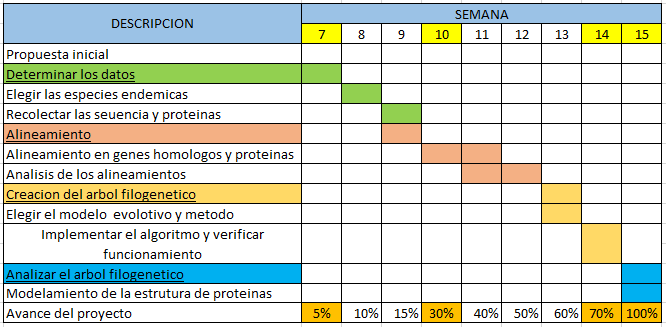
\includegraphics[width=14cm,height=8cm]{cronoextendido.png}\\
	Fig: Cronograma por semanas	
\end{center}

\begin{center}
	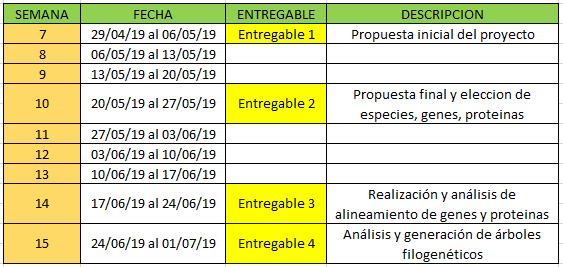
\includegraphics[width=10cm,height=6cm]{cronoentregrable.png}\\
	Fig: Cronograma coincidente a los entrégales
\end{center}


\vspace*{0.2in}


\section{Algoritmos e implementación computacional}
Una descripción de los algoritmos y herramientas que se [planean utilizar en caso de la propuesta] utilizados incluyendo pseudo código y código fuente
\section{Resultados}
Una descripción de los resultados [esperados en el caso de la propuesta]. Un reporte integrando los resultados proporcionados por la herramienta
\section{Conclusiones}
Incluye las ventajas y desventajas del enfoque utilizado, aspectos inesperados del proyecto, trabajo futuro, etc.
\section{Apéndice}


\end{document}